% -------------------------------------------------------------
% -------------------------------------------------------------
\section{Introduction}
% -------------------------------------------------------------
\subsection{Work objectives}
Why is ITER so large? How have been determined its main dimensions? Are these dimensions sufficient to reach its scientific goals,  i.e. produce 500 MW of fusion power for pulses of 400s with a power amplification ratio of 10 \footnote{\url{https://www.iter.org/sci/Goals}}? And what should be the size of tokamak fusion reactor: smaller or larger than ITER? How much additional power is required to reach positive power amplification? How does it affect the magnets and the plasma facing components? 

Answering these questions is the main motivation for this group work. During the few days dedicated to this work, you will have to answers some of these questions by working in small groups. Interactions between groups is highly encouraged: no one can be expert of all the various physical and technological fields required to build a fusion machine, so group work is essential. When necessary, results will be shared between groups.

In the first part of the work, you will derive from a 0-dimensional approach the necessary equations to deduce a couple $(R, B)$ for a given reactor project of prescribed $(P_{DT}, Q)$. By proceeding this way, some other characteristics of the plasma (namely the shape of the plasma, including elongation and aspect ratio, the average ion mass $\hat M$, the edge safety factor $q_a$ and the density $n_N$ normalised to the Greenwald density) will have to be prescribed by other considerations. This method will be applied to deduce the ITER parameters $(R, B)$. 

Each group results will be presented and shared with each others during the Part 1 evaluation. Once done, you will have to fix the main dimensions of the tokamak to be build. In the Part 2, groups will then focus on particular aspects of the machine: magnets, MHD stability, plasma facing components, safety and remote handling, external heating systems, etc. In case of problems, questions or design change requests, groups will be able to exchange between each other, or even to organise a general meeting in which topics affecting all groups can be discussed.

% -------------------------------------------------------------
\subsection{Schedule (2019)}
\begin{itemize}
\item Thursday and Friday 7 and 8th of March: Part 1
\item Monday 11th of March: groups restitution
\item From Tuesday 12th to Thursday 14th: Part 2
\item Friday 15th of March: Final groups restitution
\end{itemize}

% -------------------------------------------------------------
% -------------------------------------------------------------
\section{Derivation of the Governing Relations}
The International System of Units (SI) should be used. Quantities which are \emph{not} expressed in SI units should be emphasised with a specific symbol, for example with hats ``$\hat{...}$''. We recommend using the following alternative units: 
\begin{itemize}
    \item $\hat n$ is the density in $10^{19} \si{m^{-3}}$: 
    $\hat n = 10^{-19}\,n_{\si{[m^{-3}]}}$
    \item $\hat T$ is the temperature in $keV$: $\hat T = 10^{-3}\, k_B T_{[K]}\,/e$ \\(with $k_B \approx 1.3807\, 10^{-23} \si{J.K^{-1}}$ the Boltzmann's constant and $e\approx 1.6022\, 10^{-19}C$ the elementary electric charge)
    \item $\hat I_p$ is the plasma current in MA: $\hat I_p = 10^{-6}\,I_{p\,[A]}$
    \item $\hat P$ is the power in MW: $\hat P = 10^{-6}\, P_{[W]}$
    \item $\hat M$ is the mass in Atomic Mass Unit
\end{itemize}
When possible, try to combine all numerical values (coming from physical constants) into a single constant $C$.


\subsection{Plasma Geometry}
Let's define $a$ the minor radius and $R$ the major radius of the tore plasma. Is is also usual to define the plasma \textit{elongation} as $\kappa \doteq b/a$, $b$ being the largest radius of the ellipsoid ($\kappa=1$ for a circular cross-section, and is larger than unity for an elongated plasma.). We also define the inverse aspect ratio  as $\varepsilon  \doteq a /R$. 
\paragraph{Q:} Express the plasma volume as function of $R, \kappa$ and $\varepsilon$.

\subsection{Plasma Current}
\paragraph{Q:} Integrating the Maxwell-Ampère equation over the whole plasma cross-section, express the plasma current $\hat I_p$ as a function of $\varepsilon, q_a, R$ and $B$. 


% -------------------------------------------------------------
\subsection{Greenwald Density}
As stated in a recent topical review on the subject \cite{Greenwald2002}, \emph{``in addition to the operational limits imposed by MHD stability on plasma current and pressure, an independent limit on plasma density is observed in confined toroidal plasmas. [...] In tokamaks, [...] there is strong evidence linking the limit to physics near the plasma boundary [...]''}. As a matter of fact, the so-called \textit{Greenwald density} $n_G$ is not a sharp density limit, since discharges with peaked density profiles can well operate above this value. So far, there is no widely accepted, first principles model for the density limit. Yet, the focus is currently either on mechanisms which lead to strong edge cooling, or on collisionality enhanced turbulent transport.

From \cite[eq.(14.146)]{Freidberg2007}, the most common empirical scaling for (line-averaged) density limit is the following:
\begin{equation}
\boxed{\hat n_G \doteq C_n \frac{\hat I_p}{\varepsilon^2 R^2}  }
\label{eqn:greenwald_density}
\end{equation}
with $C_n = 10/\pi \approx 3.18$.

\paragraph{Q:} Express the Greenwald density using the expression of the plasma current given above. Note that you can introduce the normalised density $n_N\doteq n/ n_G$ in order to express the density $n$ from the Greenwald density limit.

% -------------------------------------------------------------
\subsection{Plasma Beta}
The plasma beta $\beta$ is defined as the ratio of the plasma pressure to the magnetic pressure. Assuming equal ion and electron temperatures ($T_e=T_i$).

% -------------------------------------------------------------
\subsection{Fusion Power}
To get nuclear fusion, nuclei have to come close enough to each other where nuclear forces can overcome their mutual electrostatic repulsion. This would require temperatures of the order of 720 keV for head-on collisions of thermal particles to lead to fusion reactions in a classical way. Actually, quantum physics has to be taken into account in the process. Both in tokamaks and in stars interiors, fusion reactions take place predominantly due to the tunnel effect. Crossing this barrier can be quantified in a probabilistic manner with the reaction rate $R$ $[\mathrm{reaction/m^3 s}]$, defined as the probability of reaction per unit time and volume. The reaction rate between mono-energetic ions of density $n_1$ $\mathrm{[m^{-3}]}$ striking target ions of density $n_2$ $\mathrm{[m^{-3}]}$ is proportional to the effective cross-section area $\sigma$ $\mathrm{[m^2]}$ and to the velocity difference $v_{12}$ between the two species:
\begin{equation*}
r_{12} = n_1 n_2 \; \sigma v_{12}
\end{equation*}
The quantity  $\sigma v_{12}$, which depends on the kinetic energy of the colliding particles, is called the reactivity ($\mathrm{[m^3/s]}$). Note that the reaction rate $r_{12}$ is proportional to the square of the density of the mixture. In fusion plasmas, ions are not mono-energetic. They are assumed to have Maxwellian velocity distributions. The average reactivity $\langle \sigma v \rangle_{12}$ derives from the following expression:
\begin{equation*}
\left < \sigma v \right >_{12} 
= \int_{-\infty}^{+\infty} \int_{-\infty}^{+\infty} 
\sigma(v_{12}) v_{12}\;  f_1(v_1) f_2(v_2) \; dv_1dv_2
\end{equation*}
Finally, the average reaction rate $R_{12}$ reads:
\begin{equation*}
R_{12} = n_1 n_2 \; \left < \sigma v \right >_{12}
\end{equation*}
It governs the time evolution of both densities: $dn_1/dt = dn_2/dt = -R_{12}$.
The temperature dependence of the reactivity $\langle \sigma v \rangle_{12}$ is plotted on figure \ref{fig:reactivity} for several fusion reactions (data from \cite{Huba2013}).

\begin{figure} 
\begin{center}
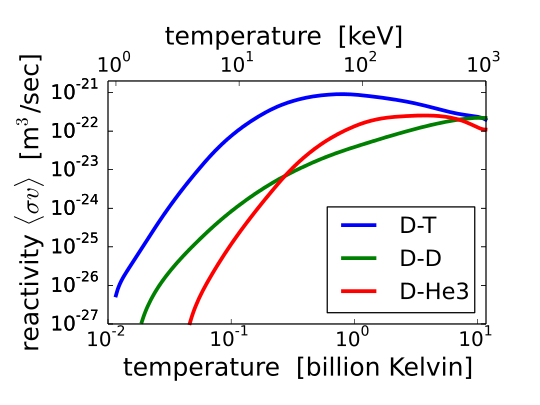
\includegraphics[width=0.75\textwidth]{figures/reactivity_DT.png}
\caption{Fusion reactivity }
\label{fig:reactivity}
\end{center}
\end{figure}

The D-T reactivity reaches its maximum for a temperature of 64 keV, corresponding to a temperature of $742\,10^6$ K. Since it has the highest reaction rate, the D-T reaction is the “easiest” to initiate (maximum reactivity at lowest temperature) of all fusion reactions and is the targeted fusion reaction \cite{FusionCEA1987}: 
\begin{equation*}
\mathrm{D + T} \longrightarrow \mathrm{{}^4 He~(3.56~MeV) + n~(14.03~MeV)}
\end{equation*}
The D-T reaction leads to a total released energy of $E_{DT}$ = 17.59 \si{MeV} = $2.82\times 10^{-12} \si{J}$ per fusion reaction. Notice that the ratio of the total energy to that carried by the alpha particles $\lambda \doteq 17.59/3.56 \approx 4.94$ is not exactly equal to 5 as one would expect on the basis of momentum conservation. Actually, this ratio \emph{is obviously} consistent with momentum conservation, as it should, provided one takes into account relativistic effects. This point is detailed in section \ref{appendix:fusion_power}.

The fusion power per unit volume $p_{DT}$ produced by the fusion of the nuclei of deuterium and tritium reads: 
\begin{equation*}
  p_{DT} = n_D n_T \left< \sigma v \right>_{DT} E_{DT}
\end{equation*}
with $n_D$ and $n_T$ the deuterium and tritium density and $\left< \sigma v \right>_{DT}$ the D-T reactivity. 

\paragraph{Q:} Assuming equal deuterium and tritium densities $n/2$ with $n$ the electron density,  a constant reactivity in the plasma (``flat profile hypothesis''), express the  fusion power as a function of the plasma geometry parameters.

In the temperature range 10.3-18.5 keV, it turns out that the reactivity $\left< \sigma v \right>_{DT}$ can well (with about 10$\%$ error) be approximated by \cite[(1.5.4)]{Wesson2004}: 
\begin{equation*}
  \left< \sigma v \right>_{DT} \approx 1.18\, 10^{-24}\; \hat T^2 \;\si{\left[m^3 s^{-1}\right]}
\end{equation*}

\paragraph{Q:}  From the previous approximation, derive the fusion power expression in MW.

Notice that the fusion power can also be expressed in terms of $\beta_N$by using the result of the previous section.

\paragraph{Q:}  How does this total fusion power is distributed among the alpha particles and the neutrons?

% ----------------------------------------------------------------
\subsection{Plasma heating and amplification factor Q}
Conversely to neutrons which leave the plasma, charged $\alpha$ nuclei are confined by the magnetic field and should ideally transfer their energy to the main ions before being extracted\footnote{There are basically 2 ways for this energy transfer. Since the collision frequency scales like the velocity difference between the colliding species to the power $-3$ ($\nu_{coll,ss'}\sim n_{s'}/\Delta v_{ss'}^3$), alpha particles transfer their energy dominantly to the electrons, which are much faster due to their low inertia. Then two routes are possible for the energy transfer from the electrons to the ions. Either via collisions, or via turbulence. In the latter case, the mediator are the electrostatic plasma waves. The relative weight of those two channels is still a matter of research.}. The total -- or net -- heating power is the sum of the auxiliary plasma heating -- including Ohmic heating -- and of alpha heating:
\begin{equation}
P_{net} \doteq P_\alpha + P_{ext}
\label{eq:net_power}
\end{equation}
The plasma amplification factor is defined as:
\begin{equation}
Q \doteq \frac{P_{DT}}{P_{ext}}
\label{eq:Q}
\end{equation}
Importantly, notice that $Q$ \emph{does not} encompass -- by far -- the entire question of the energetic efficiency of a fusion reactor. Indeed, in particular, it does neither account for the energy used for cryogenic purposes (as required by the use of superconductors) nor for the conversion factor of thermal to electric energy\footnote{This point is often misleading for the public and it is important to be factually correct. Misleading statements concerning fusion and ITER power and energy since decades have been highlighted in \url{http://news.newenergytimes.net/2017/10/06/the-iter-power-amplification-myth/}. This led directly ITER to update its public information web pages on the Q-factor (cf. \url{https://www.iter.org/newsline/-/2845}).  Cf. also the follow-up \url{http://news.newenergytimes.net/2017/12/11/evidence-of-the-iter-power-deception/}}.

\paragraph{Q:} Express the net power in terms of the fusion power and of the amplification factor. Then replace the fusion power bu the expression found in the previous section. 


%----------------------------------------------
\subsection{Power loss and energy confinement time}

The total internal energy of the plasma reads as follows:
\begin{equation*}
  W  = \int \frac{3}{2} k_B \left( n_e T_e + n_i Ti \right ) dV 
  \approx \int 3 n k_BT dV
\end{equation*}
where the integral is performed over the plasma volume. 

Here, equal ion and electron temperatures have been assumed. 

\paragraph{Q:} Assuming flat density and temperature profiles and using the expression of the volume of a torus, express the total plasma internal energy $W$ in [MW.s].



The energy confinement time $\tau_E$ is usually defined as the characteristic time at which this energy is lost from the plasma due to thermal transport\footnote{This definition excludes radiative losses. It is consistent with the one used for the ITER scaling laws, discussed in a next section.}, either by collisional conduction or by turbulent thermal convection. It is defined as $\tau_E \doteq W/P_{loss}$. 

\paragraph{Q:} Express the power lost from the plasma $P_{loss}$. Note you can also express it as a function of $\beta_N$.


%----------------------------------------------
\subsection{The triple product and the Lawson criterion}
At equilibrium, the total heating power is equal to the loss power. Using the previous definitions, this translates into $P_{net} =P_{loss}$ \footnote{Should the plasma not be at equilibrium and/or be subject to significant radiative losses in the confined region, then $P_{net}$ should be replaced by $(P_{net}-dW/dt-P_{rad})$. The subtraction of $P_{rad}$ ensures the balance equation to be consistent with the retained definition of $\tau_E$.}.

\paragraph{Q:} Using both expressions of the powers, express an expression for the so-called triple product $nT\tau_E$. Express the Lawson criterion, which corresponds to the limit when $Q\to\infty$, $i.e.$ when the entire plasma heating is provided by alpha heating ($P_{net}=P_\alpha$). For a plasma density of $\hat n=10$ (hence $n=10^{20}\si{m^{-3}}$) at the temperature of $\hat T=10$keV, what is the confinement time imposed by the Lawson criterion?


\paragraph{Q:} How does vary the amplification factor $Q$ with the energy confinement time normalised to the Lawson time?



%----------------------------------------------
\subsection{Scaling law of the energy confinement time}

Experimental results have shown that the energy time in ELMy H-mode tokamak plasmas (referred to as the ITER IPB98(y,2) scaling law \cite[eq.(20)]{ITERphysics_chap2}) is well represented -- the root means square error is about 15.6\% -- by the following scaling law:
\begin{equation*}
  \tau_E = C_{SL} \hat M^{0.19} \kappa^{0.78} \varepsilon^{0.58} 
  \hat n^{0.41} \hat I_p^{0.93} R^{1.97} B^{0.15}  \hat P_{net}^{-0.69}
\end{equation*}
with $C_{SL} = 0.0562$.
Here, $\hat I_p$ and $B$ are the plasma current and the toroidal magnetic field at the magnetic axis, respectively, $\hat n$ the line-averaged density, and $\hat M$ is the average ion mass (in Atomic Mass Unit)\footnote{Cf. also \url{http://fusionwiki.ciemat.es/wiki/Scaling_law}.}. 

\paragraph{Q:} 
Introducing the normalised density $n_N = \hat n/\hat n_G$ and replacing the current by the expression found before, recast the scaling law. 
\paragraph{Q:} One last step is to replace $\hat P_{net}$ by $\hat P_{loss}$, which is equivalent at equilibrium, and to use the expression of the pressure in terms of $\beta_N$ to obtain the expression of $(\hat n\hat T\tau_E)^{0.31}$. 

This provides an expression of $\beta_N$ as a function of $R$, $B$ and $Q$ at prescribed values of the average ion mass $\hat M$, of geometrical variables ($\kappa$ and $\varepsilon$), of the edge safety factor $q_a$ and of the normalised density $n_N$.
